\documentclass[xcolor=dvipsnames]{beamer}

\mode<presentation>
{
  \usetheme{Frankfurt}
  % or ...

  \setbeamercovered{transparent}
  % or whatever (possibly just delete it)

  %\usecolortheme[named=Brown]{structure}

}

\usepackage[english]{babel}
\usepackage[utf8x]{inputenc}
%\usepackage[latin1]{inputenc}
\usepackage{times}
\usepackage[T1]{fontenc}
\usepackage{array,booktabs,tabularx}
\newcolumntype{Z}{>{\centering\arraybackslash}X} % centered tabularx columns
\newcommand{\pphantom}{\textcolor{ta3aluminium}} % phantom introduces a vertical space in p formatted table columns??!!
\usepackage{amsmath,amsthm, amssymb, latexsym}
\usepackage{graphicx}

\title[] {Implementación HW/SW de Arquitecturas de Clasifiación de Paquetes Sobre Lógica Reconfigurable.}

\author[] {Jairo N. Trad y Luis R. Romano}


\institute[Universidades] % (optional, but mostly needed)
{
  \scriptsize Laboratorio de Comunicaciones Digitales \\
  \scriptsize Universidad Nacional de Córdoba, Facultad Ciencias Exactas, Físicas y Naturales \\ 
}

\AtBeginSubsection[]
{
  \begin{frame}<beamer>{Agenda}
    \scriptsize
    \tableofcontents[currentsection,currentsubsection]
  \end{frame}
}

% If you wish to uncover everything in a step-wise fashion, uncomment
% the following command: 

%\beamerdefaultoverlayspecification{<+->}

\begin{document}

\begin{frame}
  \titlepage
\end{frame}

\begin{frame}{Agenda}
  \tableofcontents
  % You might wish to add the option [pausesections]
\end{frame}

\scriptsize

\section{Motivación}

\subsection{Requerimientos}

\begin{frame}{Requerimientos de procesamiento en Redes}
  \scriptsize
  
  \begin{block}<+->{Características de Tráfico}

    \begin{itemize}
      \item Las redes de datos crecen en {\bf Complejidad:} nuevas aplicaciones, multimedia

      \item Las redes de datos crecen en {\bf Velocidad:} $n \times 100 Gbps\ (1Tbps@2015)$

      \item {\bf Consolidación} de múltiples servicios sobre redes Ethernet
      
      \item Redes \emph{Locales}, \emph{Metropolitanas} y \emph{Extensas} utilizan {\bf Conmutación de Paquetes}

      \item Adopción de tecnologías para \emph{virtualización} en redes y servidores
    \end{itemize}
    
  \end{block}
    
  \begin{block}<+->{Procesamiento de Paquetes}
    \begin{itemize}

      \item Los \emph{enlaces} ofrecen alta capacidad. El \emph{procesamiento} de paquetes es {\bf crítico} y debe optimizarse

      \item El rocesamiento \emph{a velocidad de línea}

      \item Paquete Ethernet mínimo $=64 bytes$ $\rightarrow 6 nanosegundos/paquete$  
    \end{itemize}    
  \end{block}

\end{frame}



\subsection{Soluciones}
\begin{frame}{Soluciones}

  \begin{block}<+->{Granularidad}  
    \begin{itemize}
      \scriptsize
      \item {\bf Actualmente} $\rightarrow$ {\bf paquetes} de longitud {\bf variable}
      \item Peor caso $\rightarrow$ mínima longitud (64 bytes en Ethernet)
      \item {\bf Tendencia} $\rightarrow$ agregación de paquetes en {\bf flujos}
      \item Ejemplos: Multi-protocol Label Switching (MPLS), VLANs (802.1Q)  
    \end{itemize}
  \end{block}
    
  \vskip2ex  
%    \newcolumntype{V}{>{\centering\arraybackslash} m{.4\linewidth} }
    \begin{tabularx}{\linewidth}{ZZ}
%    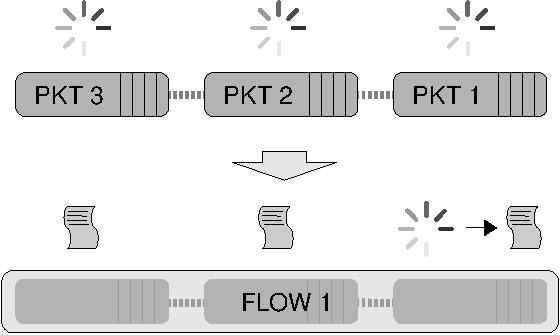
\includegraphics[scale=0.45]{figures/packet_vs_flow-crop} 
    &
%    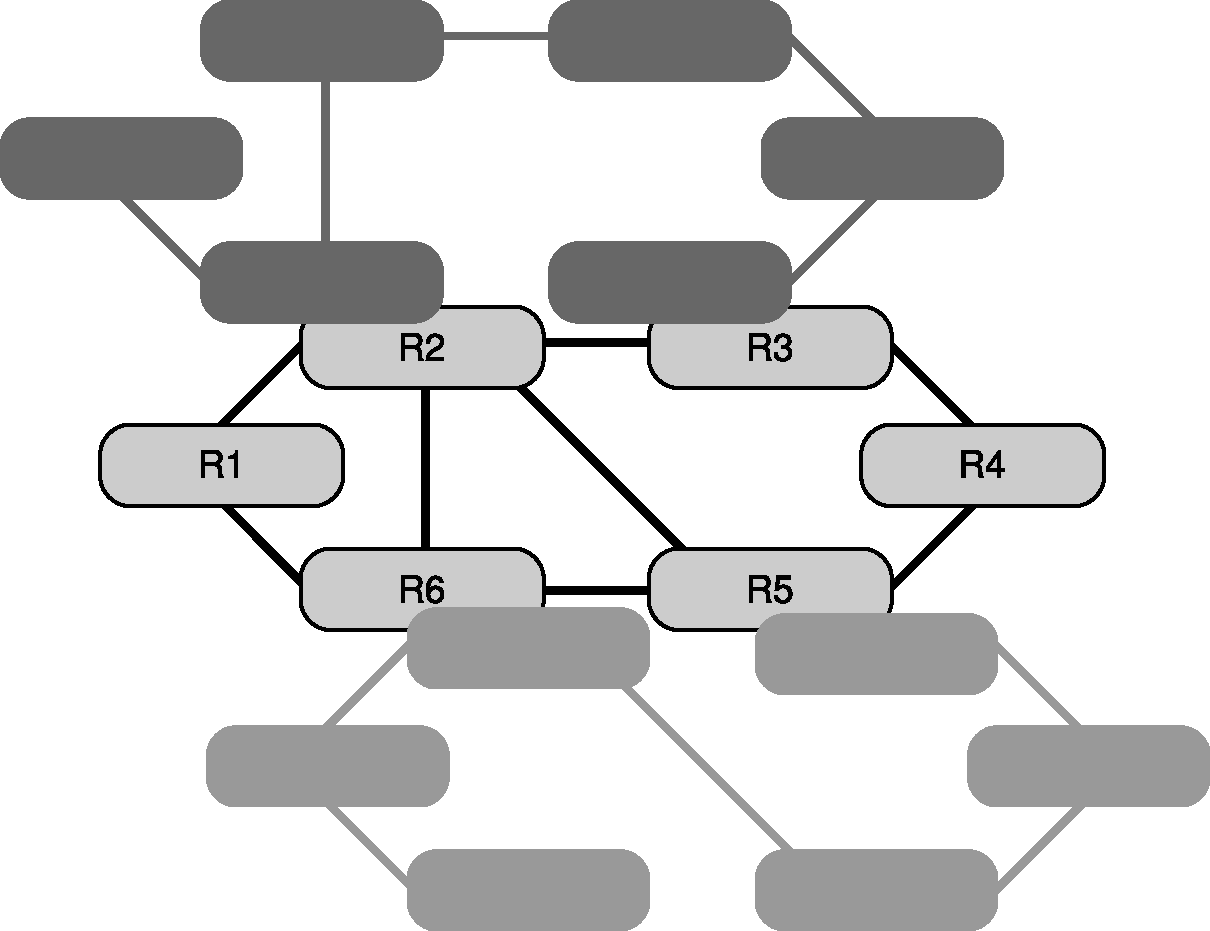
\includegraphics[scale=0.2]{figures/network_virtualization_2}
    \\
    \tiny Agregacion de flujos
    &
    \tiny Virtualizacion de redes
    \\
  \end{tabularx}


\end{frame}  
  
   
\begin {frame}{Tecnologías Actuales}   
  
  Requerimientos $\rightarrow$ {\bf flexibilidad, performance} 
  
  \begin{block}<+->{Circuitos de Propósito Específico (ASICs)} 
    \begin{itemize}
      \scriptsize
      \item Cientos de bloques especializados trabajando en paralelo
      \item Alto desempeño. No programables, alto costo y tiempo de desarrollo.
    \end{itemize}
  \end{block}

  \begin{block}<+->{Network Processors (NPs)}   
    \begin{itemize}
      \scriptsize
      \item Múltiples elementos de procesamiento, buena performance para ciertas tareas. IXP(Intel), PowerNP (IBM)
      \item Difícil portabilidad, interfaces propietarias
    \end{itemize}
  \end{block}

  \begin{block}<+->{Procesadores de Propósito General (GPPs)} 
    \begin{itemize}
      \scriptsize
      \item Arquitectura PC + Software especializado: \emph{Click}, \emph{Zebra/Xorp/Quagga}
      \item Alta flexibilidad, bajo costo. Limitación por transacciones con RAM y naturaleza secuencial
    \end{itemize}
  \end{block}
  
\end{frame}


\begin{frame}{Nuevas tecnologías}

  \begin{block}<+->{Dispositivos Lógicos Programables (FPGAs)} 
    \begin{itemize}
      \scriptsize
      \item Permiten \emph{reconfiguración} y \emph{reprogramación}, contando con librerías de \emph{Open Hardware}. 
      \item Su performance no es lejana a la de un ASIC. Fabricantes: Altera, Xilinx, Actel.
      \item Incorporación creciente de bloques \emph{hardcore} especializados
    \end{itemize}      
  \end{block}
    \vskip3ex
    \center 
    \newcolumntype{V}{>{\centering\arraybackslash} m{.3\linewidth} }
    \begin{tabularx}{\linewidth}{VVV}
%      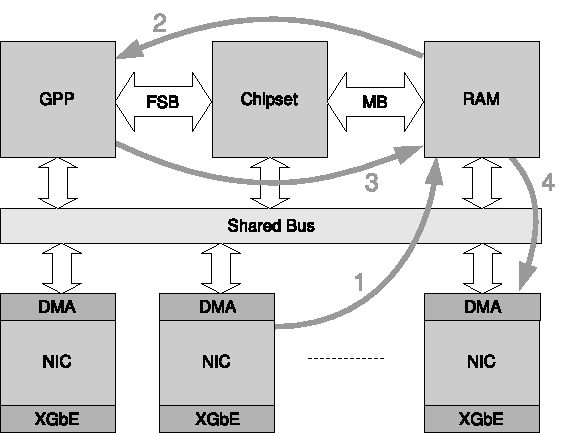
\includegraphics[scale=0.35]{figures/GPP_based}
      &
%      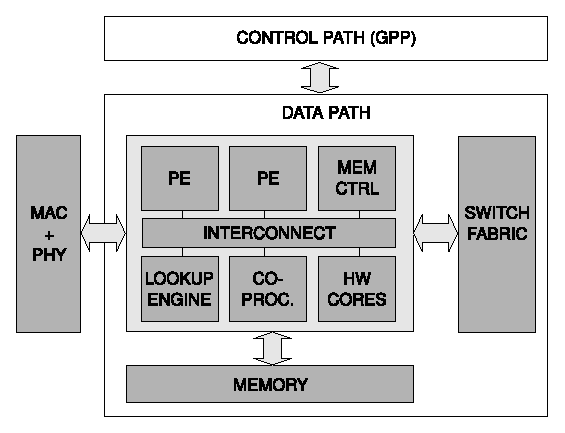
\includegraphics[scale=0.35]{figures/NP_based}
      &
%      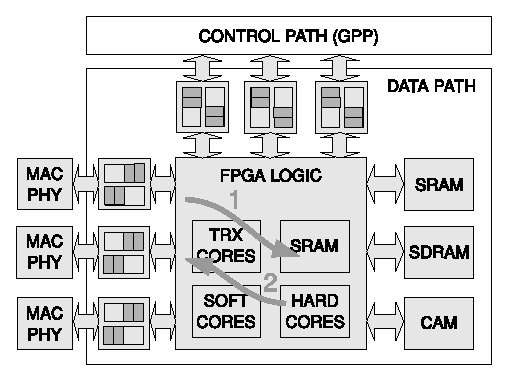
\includegraphics[scale=0.38]{figures/FPGA_based}
      \\
      \tiny Implementación con GPPs
      &
      \tiny Implementación con NPs
      &
      \tiny Implementación con FPGAs
      \\
    \end{tabularx}
\end{frame}

\subsection{Problema marco}
\begin{frame}{Clasificación de Paquetes}

 \begin{block}<+->{Clasificación}   
    \begin{itemize}
      \scriptsize
      \item La necesidad de procesar cada vez más paquetes de datos lleva a lo que se conoce como \textit{clasificación.}
      \item Es el proceso de categorización de paquetes en distintos flujos.
      \item Efectuada en base a un número de campos de una cabecera.
      \item En general, para una clasificación basada en N campos, se dice que la misma es N-dimensional (o multidimensional) 
      \item Un caso en particular de la clasificación unidimensional (N=1) es lo que se conoce como \textit{lookup}.     
    \end{itemize}
  \end{block}

\end{frame}

\begin{frame}{LookUp}

 \begin{block}<+->{Lookup}   
    \begin{itemize}
      \scriptsize
      \item Se lleva a cabo en el dispositivo de enrutamiento.
      \item Un paquete llega por una interfaz de entrada. Éste porta una dirección IP determinada.
      \item El dispositivo consulta una tabla de forwardeo para determinar la interfaz de salida para el paquete en cuestión
      \item Dicha tabla contiene un conjunto de prefijos con sus correspondientes interfaces de salida.
      \item El paquete es correspondido con el prefijo más largo que esté contenido en la dirección de destino y luego es redirigido  a la correspondiente interfaz de salida.
   
    \end{itemize}
  \end{block}

\end{frame}

\subsection{Objetivos}
\begin{frame}{Objetivos}
\begin{block}<+->{Generales}   
    \begin{itemize}
      \scriptsize
      \item Estudiar las diversas arquitecturas de clasificacion de paquetes para poder encontrar las limitaciones en la implementacion de las mismas tanto en software como en hardware. 
      \item Ganar conocimiento acerca las diversas posibilidades que ofrecen las FPGA para la implementacion de este tipo de algoritmos y las opciones con las que se cuenta a la hora de implementar un sistema embebido en este tipo de dispositivos.
    \end{itemize}
  \end{block}
  
 \begin{block}<+->{Específicos}   
    \begin{itemize}
      \scriptsize
     \item Implementar un sistema embebido que realice la clasificiación unidimensional de paquetes mediante una arquitectura mixta, Hardware-Software, en lógica reprogramable y que permita contratastar algunos de los algoritmos de clasificacion existentes. 
	\item Implementar como mínimo dos algoritmos de clasificación. 
	\item Mejorar las algoritmos anteriormente mencionados, poniendo el foco en optimizar el código.
   
    \end{itemize}
  \end{block}
 \end{frame}

\section{Sistema}
\subsection{Solución Propuesta}
\begin{frame}{Solución}

... Diagrama de bloques ...

\end{frame}

\subsection{Descripcion funcional de cada bloque}
\begin{frame}{Descripcion funcional}
\begin{block}<+->{Microprocesador}   
    \begin{itemize}
      \scriptsize
     	\item
    \end{itemize}
  \end{block}
  \begin{block}<+->{Bus de interconexión}   
    \begin{itemize}
      \scriptsize
     	\item
    \end{itemize}
  \end{block}
\end{frame}
\begin{frame}{Descripcion funcional}
\begin{block}<+->{Memoria}   
    \begin{itemize}
      \scriptsize
     	\item
    \end{itemize}
  \end{block}
  \begin{block}<+->{Dispositivos de E/S}   
    \begin{itemize}
      \scriptsize
     	\item
    \end{itemize}
  \end{block}
\end{frame}

\subsection{Algoritmos de Clasificación}
\begin{frame}{Algoritmos de Clasificación}
\begin{block}<+->{Linear Lookup (LLU)}   
    \begin{itemize}
      \scriptsize
     	\item Prefijos almacenados en una lista enlazada
	\item Se toma como entrada una determinada dirección de destino y se va comparando nodo a nodo.
	\item Prefijos ordenados por longitud
	\item La primer coincidencia es la mejor
    \end{itemize}
  \end{block}
  \begin{block}<+->{Unibit trie lookup (UTL)}   
    \begin{itemize}
      \scriptsize
     	\item Prefijos almacenados en un arbol
	\item Cada nodo representa un bit del prefijo
	\item Se toma como entrada una dirección de destino y se va recorriendo el arbol en base a los bits
    \end{itemize}
  \end{block}
\end{frame}

\subsection{Modulo extractor de cabeceras}
\begin{frame}{Modulo extractor de cabeceras}
\begin{block}<+->{Descripción funcional}   
    \begin{itemize}
      \scriptsize
     	\item
    \end{itemize}
  \end{block}
  \begin{block}<+->{Formato de la cabecera}   
    \begin{itemize}
      \scriptsize
     	\item
    \end{itemize}
  \end{block}
\end{frame}

\section{Arquitectura}
\subsection{Diagrama en bloques: Lineas E/S}
\begin{frame}{Diagrama en bloques: Lineas E/S}

---aqui el diagrama ...

\end{frame}

\begin{frame}{Arquitectura}
  \begin{block}<+->{Interfaz Avalon MM}   
    \begin{itemize}
      \scriptsize
     	\item
    \end{itemize}
  \end{block}
\end{frame}

\section{Implementación}
\subsection{NIOS II}
\begin{frame}{Microprocesador NIOS II}
  \begin{block}<+->{NIOS II}   
    \begin{itemize}
      \scriptsize
     	\item
    \end{itemize}
  \end{block}
\end{frame}

\subsection{Herramientas / Recursos Utilizados}
\begin{frame}{Herramientas / Recursos Utilizados}
\begin{block}<+->{Quartus}   
    \begin{itemize}
      \scriptsize
     	\item IDE de Altera
	\item Incluye editor de textos y herramientas para síntesis
	\item Lenguaje HDL utilizado: Verilog HDL
    \end{itemize} 
  \end{block}
  \begin{block}<+->{Eclipse IDE for NIOS}   
    \begin{itemize}
      \scriptsize
     	\item Version de la IDE Eclipse adaptada para trabajar con el microprocesador NIOS II
    \end{itemize}	
  \end{block}
\end{frame}

\subsection{Verificación}
\begin{frame}{Verificación}
\begin{block}<+->{Etapas}   
    \begin{itemize}
      \scriptsize
     	\item 1º Paso: Módulo más simple (simpleRW)
     	\item 2º Paso: Implementación del modulo extractor. Debugging de señales.
     	\item 3º Paso: Integración extractor-software. LLU y UTL.
    \end{itemize}
  \end{block}
\end{frame}

\section{Resultados}
\subsection{Introducción}
\begin{frame}{Introducción}
  \begin{block}<+->{Presentación de los resultados}   
    \begin{itemize}
      \scriptsize
     	\item     	
    \end{itemize}
  \end{block}
\end{frame}

\subsection{Caso algoritmos unicamente}
\begin{frame}{Caso algoritmos unicamente} 
 .. Grafico correspondiente ...
\end{frame}

\subsection{Caso loopback}
\begin{frame}{Caso loopback} 
 .. Grafico correspondiente ...
\end{frame}

\subsection{Implementacion completa}
\begin{frame}{Implementación completa: LLU} 
 .. Graficos retardo mínimo ...
\end{frame}


\begin{frame}{Implementación completa: LLU} 
 .. Graficos retardo promedio ...
\end{frame}


\begin{frame}{Implementación completa: LLU} 
 .. Graficos retardo máximo ...
\end{frame}


\begin{frame}{Implementación completa: UTL} 
 .. Graficos retardo mínimo ...
\end{frame}


\begin{frame}{Implementación completa: UTL} 
 .. Graficos retardo promedio ...
\end{frame}


\begin{frame}{Implementación completa: UTL} 
 .. Graficos retardo máximo ...
\end{frame}

\subsection{Comparativa inter-algortimos}
\begin{frame}{Comparativa inter-algortimos} 
 .. Grafico comparativo ...
\end{frame}

\section{Conclusiones}
\begin{frame}{Conclusiones} 
\begin{block}<+->{Conclusiones}   
    \begin{itemize}
      \scriptsize
     	\item     	
    \end{itemize}
  \end{block}
\end{frame}

\end{document}
